\hypertarget{free-energy-perturbation-using-biosimspace}{%
\section{Free Energy Perturbation using
BioSimSpace}\label{free-energy-perturbation-using-biosimspace}}

Authors:

\begin{itemize}
\tightlist
\item
  Jenke Scheen - j.scheen@sms.ed.ac.uk
\item
  Julien Michel
\end{itemize}

\hypertarget{introduction}{%
\subsection{Introduction}\label{introduction}}

Computational chemists can support structure-activity relationship
studies in medicinal chemistry by making computer models that can
predict binding affinity of ligands to proteins. One of the most popular
techniques for this is Free Energy Perturbation (FEP), which relies on
simulation alchemical transformations of ligands in a congeneric series,
simulating them both in a protein target and in just a waterbox.
Relative free energies of binding (ΔΔG in kcal/mol) can then be computed
by simply subtracting the ΔG (in protein) and the ΔG (in water). Some
introductory reading:

\href{https://www.livecomsjournal.org/article/18378-best-practices-for-alchemical-free-energy-calculations-article-v1-0}{Best
Practices for Alchemical Free Energy Calculations}

\href{https://pubs.acs.org/doi/10.1021/acs.jcim.7b00564}{Relative
Binding Free Energy Calculations in Drug Discovery: Recent Advances and
Practical Considerations}

\href{https://pubs.acs.org/doi/10.1021/acs.jcim.0c00165}{Assessment of
Binding Affinity via Alchemical Free-Energy Calculations}

This documentation will outline the steps needed to:

\begin{itemize}
\tightlist
\item
  Select a series of transformations to simulate using LOMAP
\item
  Use BioSimSpace to set up files needed for a standard FEP run in both
  SOMD and GROMACS
\item
  Run FEP using BioSimSpace on a computing cluster
\item
  Analyse FEP simulation results
\item
  Compile all FEP results locally and perform data analyses
\end{itemize}

For this tutorial we will be using TYK2, a common benchmarking set in
the FEP field, first used by Schrödinger in their
\href{https://pubs.acs.org/doi/abs/10.1021/ja512751q}{2015 FEP+ paper}.

\begin{figure}
\centering
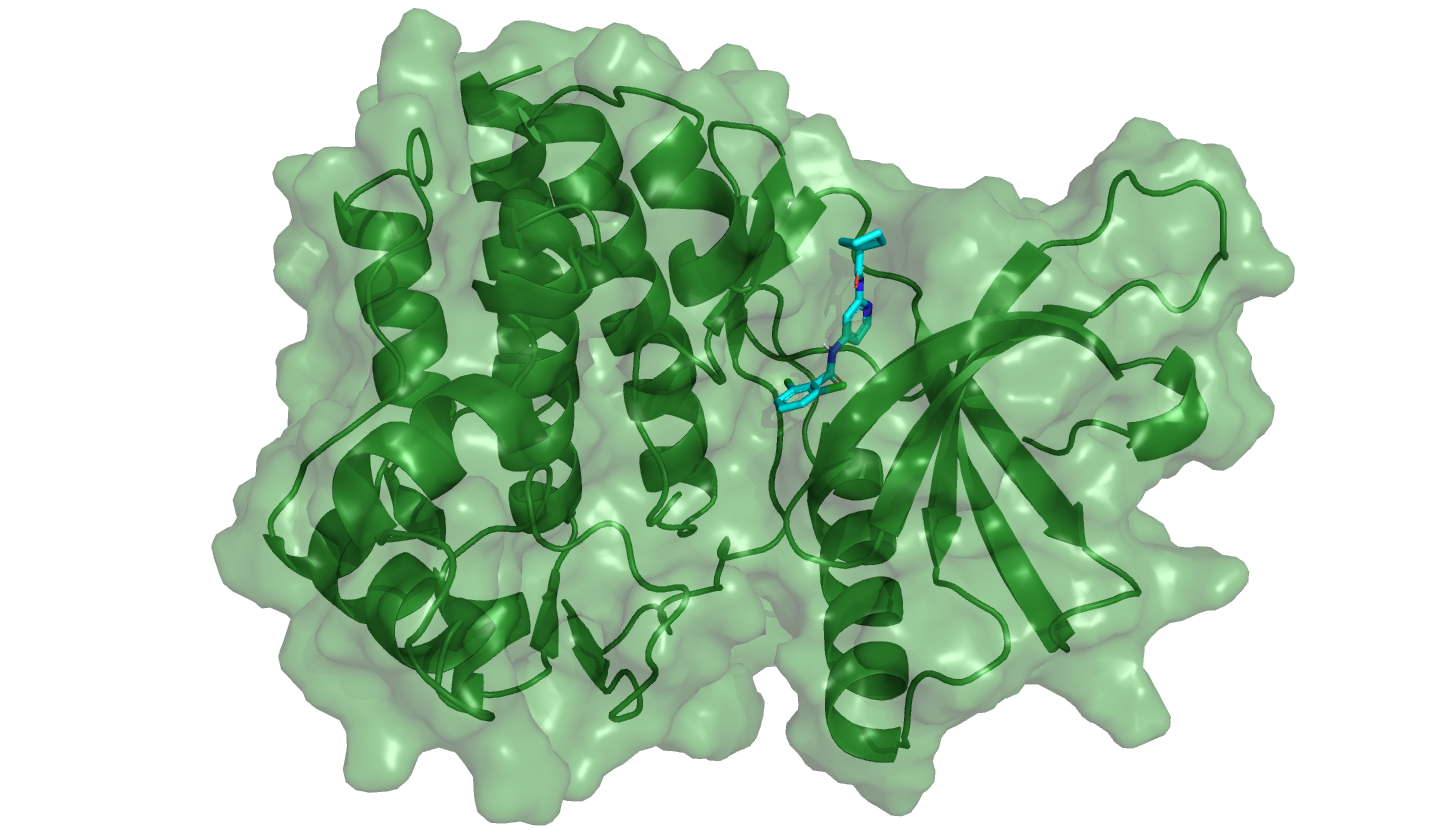
\includegraphics{./inputs/tut_imgs/tyk2_protlig.png}
\caption{image-20210416115353759}
\end{figure}

​ \emph{Figure 1: Tyrosine kinase 2 (TYK2) structure with bound ligand
(ejm\_48).}

Typically in FEP the goal is to predict free energies of binding for a
collection of ligands (normally 10-20). Although methods exist (such as
absolute FEP) that can predict these energies directly (i.e.~ΔGbind),
these are often complicated and computationally expensive. (relative)
FEP uses a basic rule in thermodynamics that dictates that, given a
thermodynamic cycle, the net energy must always be 0. FEP allows users
to compute the ΔΔG of binding between two ligands through this mechanism
(see figure 2).

\emph{Figure 2: Thermodynamic cycle that allows FEP practicioners to
compute relative energies of binding. Because the difference between the
vertical legs equals the difference between the horizontal legs, we can
circumvent predicting dGbind directly, but instead compute ddGbind by
transforming between two ligands in both the solvated and bound phase.}

Because we calculate \emph{relative} energies, we therefore have to
transform the between pairs of ligands in both the fee and bound phase
(hence the name free energy \emph{perturbation}. Typically, smaller
(i.e.~fewer heavy atoms) transformations are more reliable which means
that for a ligand series we want to selectively make combinations of
ligands to cover the whole series. In FEP, we do this using
\emph{perturbation networks}, typically generated by FEP softwares.
Although generate these networks can be done by hand, it is typically
better to do it programmatically to save time and create better networks
(transformation reliability does not depend just on transformation size,
but also a series of other unfavourable moiety transformations).

\hypertarget{setting-up-a-fep-calculation-using-biosimspace}{%
\subsection{Setting up a FEP calculation using
BioSimSpace}\label{setting-up-a-fep-calculation-using-biosimspace}}

BioSimSpace allows users to set up and run a FEP calculation in just a
few lines of code (and input files). First, we import BioSimSpace and
our input files:

\begin{Shaded}
\begin{Highlighting}[]
\ImportTok{import}\NormalTok{ BioSimSpace }\ImportTok{as}\NormalTok{ BSS}
\NormalTok{ligand_1 }\OperatorTok{=}\NormalTok{ BSS.IO.readMolecules(}\StringTok{"ligand_1.mol2"}\NormalTok{)[}\DecValTok{0}\NormalTok{]}
\NormalTok{ligand_2 }\OperatorTok{=}\NormalTok{ BSS.IO.readMolecules(}\StringTok{"ligand_2.mol2"}\NormalTok{)[}\DecValTok{0}\NormalTok{]}
\NormalTok{protein }\OperatorTok{=}\NormalTok{ BSS.IO.readMolecules(}\StringTok{"protein.*"}\NormalTok{)[}\DecValTok{0}\NormalTok{]}
\end{Highlighting}
\end{Shaded}

Parameterise our input molecules:

\begin{Shaded}
\begin{Highlighting}[]
\NormalTok{ligand_1 }\OperatorTok{=}\NormalTok{ BSS.Parameters.gaff2(ligand_1).getMolecule()}
\NormalTok{ligand_2 }\OperatorTok{=}\NormalTok{ BSS.Parameters.gaff2(ligand_2).getMolecule()}
\NormalTok{protein }\OperatorTok{=}\NormalTok{ BSS.Parameters.ff14sb(protein).getMolecule()}
\end{Highlighting}
\end{Shaded}

Because we are transforming one ligand to the other, we need them to be
well aligned. This can simply be done by:

\begin{Shaded}
\begin{Highlighting}[]
\NormalTok{atom_mapping }\OperatorTok{=}\NormalTok{ BSS.Align.matchAtoms(ligand_1, ligand_2)}
\NormalTok{ligand_1 }\OperatorTok{=}\NormalTok{ BSS.Align.rmsdAlign(ligand_1, ligand_2, atom_mapping)}
\end{Highlighting}
\end{Shaded}

Now we have to create a `merged' molecule, i.e.~a molecule that we can
transform in a way such that the endpoints are both input ligands:

\begin{Shaded}
\begin{Highlighting}[]
\NormalTok{merged }\OperatorTok{=}\NormalTok{ BSS.Align.merge(ligand_1, ligand_2)}
\end{Highlighting}
\end{Shaded}

Next, we can add this merged structure into our protein by addition:

\begin{Shaded}
\begin{Highlighting}[]
\NormalTok{system }\OperatorTok{=}\NormalTok{ merged }\OperatorTok{+}\NormalTok{ protein}
\end{Highlighting}
\end{Shaded}

Then, we put a water box around the system.

\begin{Shaded}
\begin{Highlighting}[]
\NormalTok{system_solvated }\OperatorTok{=}\NormalTok{ BSS.Solvent.tip3p(molecule}\OperatorTok{=}\NormalTok{system, box}\OperatorTok{=}\DecValTok{3}\OperatorTok{*}\NormalTok{[}\DecValTok{10}\OperatorTok{*}\NormalTok{BSS.Units.Length.nanometer])}
\end{Highlighting}
\end{Shaded}

At which point we are ready to run FEP! We just have to set how we want
to run FEP (here, just use the standard settings):

\begin{verbatim}
protocol = BSS.Protocol.FreeEnergy()
\end{verbatim}

And then we can let BioSimSpace set up all necessary files for us by:

\begin{Shaded}
\begin{Highlighting}[]
\NormalTok{freenrg }\OperatorTok{=}\NormalTok{ BSS.FreeEnergy.Binding(solvated, protocol, work_dir}\OperatorTok{=}\StringTok{"output"}\NormalTok{)}
\end{Highlighting}
\end{Shaded}

Running the FEP calculation is simply done running:

\begin{Shaded}
\begin{Highlighting}[]
\NormalTok{freenrg.run()}
\end{Highlighting}
\end{Shaded}

This only makes sense on a workstation with GPUs or GPU cloud resources
or a GPU cluster. Once the run has finished, we can analyse our FEP
results with:

\begin{Shaded}
\begin{Highlighting}[]
\NormalTok{freenrg.analyse()}
\end{Highlighting}
\end{Shaded}

\hypertarget{workflow-of-a-biosimspace-fep-pipeline}{%
\subsection{Workflow of a BioSimSpace FEP
pipeline}\label{workflow-of-a-biosimspace-fep-pipeline}}

Because a single FEP simulation typically takes 5-10 hours to run on a
single GPU (depending on settings and hardware), FEP is usually run on a
computing cluster (or HPC/ cloud service). This allows practicioners to
run many simulations at the same time, turning an FEP campaign into a
process that takes just several days (or even less) instead of weeks (or
even more).

Given a protein input file and a series of ligand input files, we will
be using a Jupyter Notebook that uses LOMAP to generate a perturbation
network for us. This notebook will also write all files necessary to
further prepare our FEP simulations. Because preparing ligands and
proteins for FEP can already require some heavy computation, this will
be the first process that will run on a cluster. Then, after running and
processing the FEP outputs, we can download the results back to our
local workstation. There, the analysis notebook uses FreeEnergyAnalysis
to process FEP predictions and generate plots.

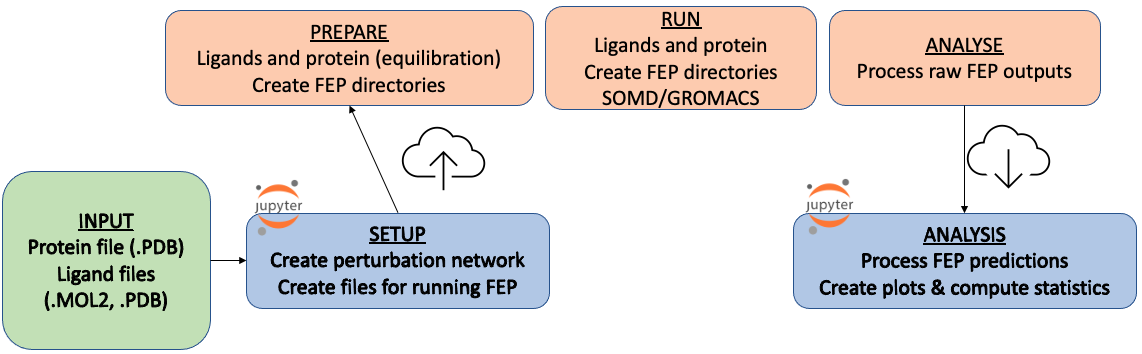
\includegraphics{./inputs/tut_imgs/fep_pipeline.png}\emph{Figure 3:
Schematic of the FEP pipeline in this report. Whereas blue boxes
represent notebooks run on a local machine, orange boxes represent
python scripts run sequentially on a computing cluster.}

\hypertarget{generating-a-perturbation-network-to-run-fep-on-a-congeneric-series-of-ligands}{%
\section{1. Generating a perturbation network to run FEP on a congeneric
series of
ligands}\label{generating-a-perturbation-network-to-run-fep-on-a-congeneric-series-of-ligands}}

For this step, open the jupyter notebook \textbf{setup\_fep.ipynb}. If
you would like to use your own ligands and protein, you can put these in
\texttt{inputs/ligands/} and \texttt{inputs/protein/}, respectively.

After running all the cells in this notebook, the folder
\texttt{./execution\_model/} will contain everything needed to run FEP
in parallel on your cluster. To move this folder to your cluster, you
can use for instance SCP:

\begin{figure}
\centering
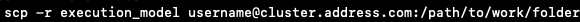
\includegraphics{./inputs/tut_imgs/scp_bash_line.png}
\caption{image-20210430143624001}
\end{figure}

\emph{Note: on some system setups, no copying will be needed as your
computing cluster might be on the same file system as your local
workstation.}

\hypertarget{running-fep-on-a-computing-cluster-using-biosimspace}{%
\section{2. Running FEP on a computing cluster using
BioSimSpace}\label{running-fep-on-a-computing-cluster-using-biosimspace}}

The folder \texttt{./execution\_model/} contains several scripts and
folders, of which the most important are:

\begin{itemize}
\tightlist
\item
  \texttt{processFEP-slurm.sh} and \texttt{processFEP-lsf.sh}: running
  either of these scripts will submit all simulations (depending on the
  cluster setup). Note that there are several parameters at the top of
  these scripts that have to be set (by e.g.~your system administrator)
  that will tell BioSimSpace of all relevant paths to software
  dependencies and other important things.
\item
  \texttt{./scripts/} contains all necessary scripts to run FEP with
  BioSimSpace. Advanced users can tweak more settings in these.
\end{itemize}

If everything has been set up correctly, running:

\begin{figure}
\centering

\includegraphics{./inputs/tut_imgs/submit_command.png}
\caption{image-20210430144209198}
\end{figure}

will start the whole FEP job submission. First, all systems will be
prepared, then run and then analysed (see figure 3). When all jobs are
finished (or when the first perturbation has finished), FEP predictions
will be written to \texttt{./outputs/SOMD/summary.csv} (in case of SOMD
engine). Logfiles for seeing process outputs can be found in
\texttt{./logs/}. Additionally, perturbations that were simulated
successfully will have an \emph{overlap matrix} figure saved to
\texttt{./logs/}; these can be checked to see if convergence was reached
per simulation leg (see
\href{https://www.livecomsjournal.org/article/18378-best-practices-for-alchemical-free-energy-calculations-article-v1-0}{Best
Practices for Alchemical Free Energy Calculations} ).

For our final analysis, we will only need
\texttt{./outputs/SOMD/summary.csv}. Thus, we need to download this file
back onto our local workstation. We can do this with SCP again, by
running (from our workstation, i.e.~not logged into the cluster):

\begin{figure}
\centering

\includegraphics{./inputs/tut_imgs/download_command.png}
\caption{image-20210430144734407}
\end{figure}

\hypertarget{analysing-fep-results}{%
\section{3. Analysing FEP results}\label{analysing-fep-results}}

For this step, open the jupyter notebook \textbf{analyse\_fep.ipynb}.
Running cells in this notebook will generate typical FEP figures
(barplots and scatterplots); if you have missing or failed
perturbations, the script should be able to work out an optimal
prediction (although at some point with enough missing FEP predictions,
ligands will of course be missing). If you happen to have experimental
affinity values, you can validate how accurate your FEP predictions are.

An example result from this notebook is the classic barplot:

\begin{figure}
\centering
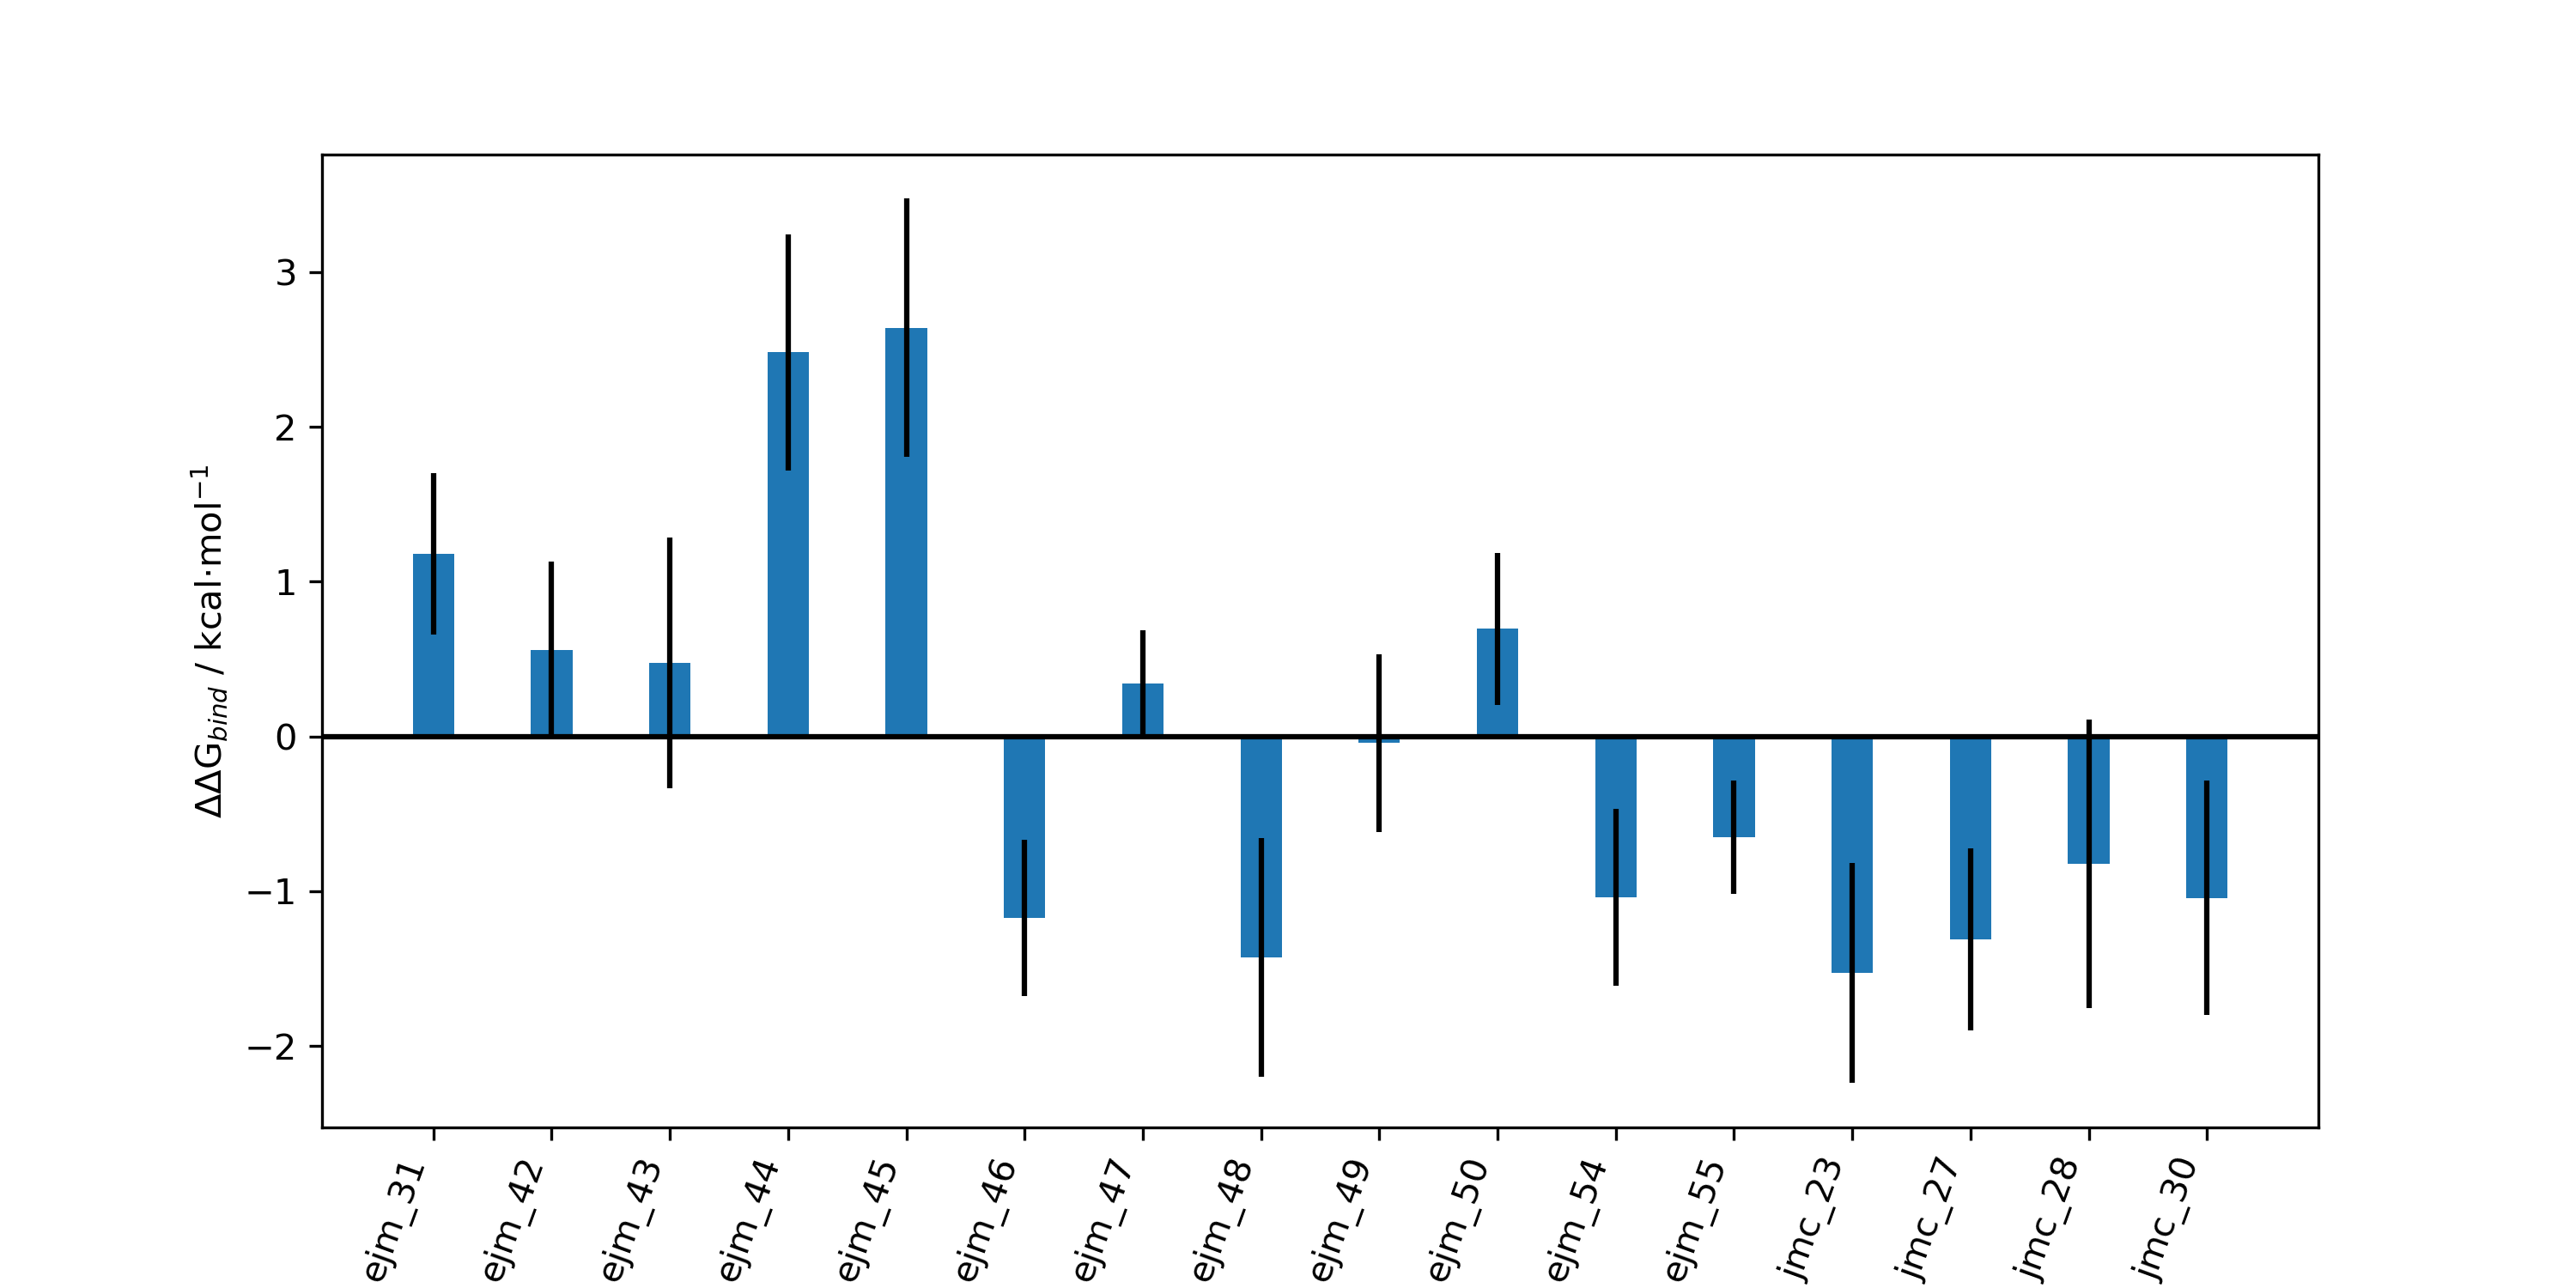
\includegraphics{./inputs/tut_imgs/fep_barplot.png}
\caption{image-20210505085226743}
\end{figure}
